%!TEX root = dippa.tex
%%% This file contains the results section of my master's thesis.
%%% Author: Viljami Aittomäki

\section{Results}


\subsection*{Quality control}

The protein and mRNA expression data appeared reasonably uniform
and mRNA data were approximately normally distributed, but several protein variables had
long tails and a few had significant outliers. 28 of the protein variables had
values that were further than 5 standard deviations away from the mean (highly
unlikely assuming normal distribution) and proteins CDK1, ERRFI1, and PIK3CA
had one value over 8 standard deviations away from the mean. These are
visually most apparent in the scaled data shown in Figure
\label{fig:protein-scaled-variable-boxplot}.

miRNA microarrays had strongly bimodal distributions with a gap between the
modes, many miRNA variables were highly skewed towards very small expression
values, and there appeared to be some quantification artifacts in the miRNA
data (see Figures \ref{fig:qc-mirna-boxplot} and \ref{fig:qc-mirna-density}).
This raises suspicion of significant noise in the miRNA data, actual miRNA
abundances should not have such a clear gap in their distribution, and values
below the gap possibly corresponded to miRNAs not actually expressed in the
data. miRNA variables that had bimodal distributions could signify that these
miRNAs are not expressed in some of the breast tumor types in the data.

No significant hospital batch effect was apparent in the data. The samples
collected at the different hospitals did not cluster into separate groups in
principal component analysis (shown in Figure \ref{fig:qc-pca}) or
hierarchical clustering (not shown) of any of the three data types.
All quality control plots are available in Appendix \ref{app:qc-plots}.




\subsection*{Correlation analysis}

Correlation between protein and mRNA expression was low on average. Protein-
mRNA correlation was clearly higher for gene-matched pairs (that is protein
and mRNA expression corresponding to the same gene) than unmatched pairs,
however, even the gene-matched correlations were quite low, with mean
$\bar{\rho} \approx 0.37$. Using the squared correlation coefficient $\rho^2$
as a measure of explained variance, the amount of protein variance explained
by the matched mRNA ranged from 0\% to 82\% with a mean of 21\%. Distributions
of Pearson correlation for matched and unmatched protein-mRNA pairs are shown
in Figure \label{fig:protein-gene-cor}.

\begin{figure}[!h]
  \centering
  \begin{subfigure}{.45\textwidth}
    \subcaption{ \label{fig:protein-gene-cor}}
    \centering
    \includegraphics[width=1\linewidth]{figures/correlationPlots/protein-gene-correlation.pdf}
  \end{subfigure}
  \begin{subfigure}{.45\textwidth}
    \subcaption{ \label{fig:gene-mirna-cor}}
    %\centering
    \includegraphics[width=1\linewidth]{figures/correlationPlots/gene-mirna-correlation.pdf}
  \end{subfigure}
  \begin{subfigure}{.45\textwidth}
    \subcaption{ \label{fig:protein-mirna-cor}}
    \centering
    \includegraphics[width=1\linewidth]{figures/correlationPlots/protein-mirna-correlation.pdf}
  \end{subfigure}

  \caption{Distributions of Pearson correlations between variables of different expression data types.
  The distributions are trimmed at the smallest and largest values.
  (a) Correlation between protein and mRNA pairs, where "matched" refers to correlating
  protein and mRNA from the same gene. Matched pairs tended to have higher correlations, but
  the correlations were low, nonetheless.
  (b) Correlation between protein and miRNA pairs, where "validated" refers to the gene
  being a validated target of the miRNA (according to TarBase),
  and "random" to a randomly picked group of protein-miRNA pairs.
  (c) Correlation between mRNA and miRNA pairs,
  where grouping is the same as in (b). There was no difference between
  validated target pairs and random pairs in (b) and (c).}
  \label{fig:correlations}
\end{figure}

Correlations between miRNAs and their validated target genes were not
significantly different from random gene-miRNA pairs (data shown in
Figure \label{fig:gene-mirna-cor}).
The validated target pairs showed no preference towards negative (or positive)
correlation. There was virtually no difference in correlations between validated
targets and randomly picked gene-miRNA pairs, contrary to what might be
expected. These finding were replicated when comparing miRNA and protein data
(Figure \label{fig:protein-mirna-cor}).




\subsection*{Model simulations}

Simulations for the cross validation (to determine model size) lasted
between 4 to 6 hours (on a computing-cluster node with 2 12-core Xeon E5 2680
2.50GHz processors), and simulations for the final projected models lasted
between 2 to 45 minutes, depending on the chosen model size. All parameters for all
simulations had low potential scale reduction $\hat{R}^2 < 1.1$, indicating
good convergence of simulation chains \citep{Gelman2013}.

The parameters for the model-size criterion, $\alpha$ and $\gamma$, had a
significant effect on the resulting model sizes and the number of models
found. Model-size distributions for several parameter values are shown in
Appendix \ref{app:model-sizes}. Values $\alpha = 0.50$ and $\gamma = 0.2$ were
chosen in order to get a projected model for most genes and to keep models
relatively sparse. This choice was, however, largely subjective.

A projected model was found for 74 genes out of the
105 genes in the data. For the rest, no miRNA variables were included in the model
for 27 genes, and the model-size criterion was met in under 200 variables for 4 genes.
Figure \ref{fig:forward-search} shows the predictive performance during the
forward search in cross validation for one of the best performing models (\emph{CDH3})
and one for which no model was found (\emph{PIK3CA}). A table of properties for the
final projected models is available in Appendix \ref{app:model-table}.

\begin{figure}[!h]
  \centering
  \begin{subfigure}{.48\textwidth}
    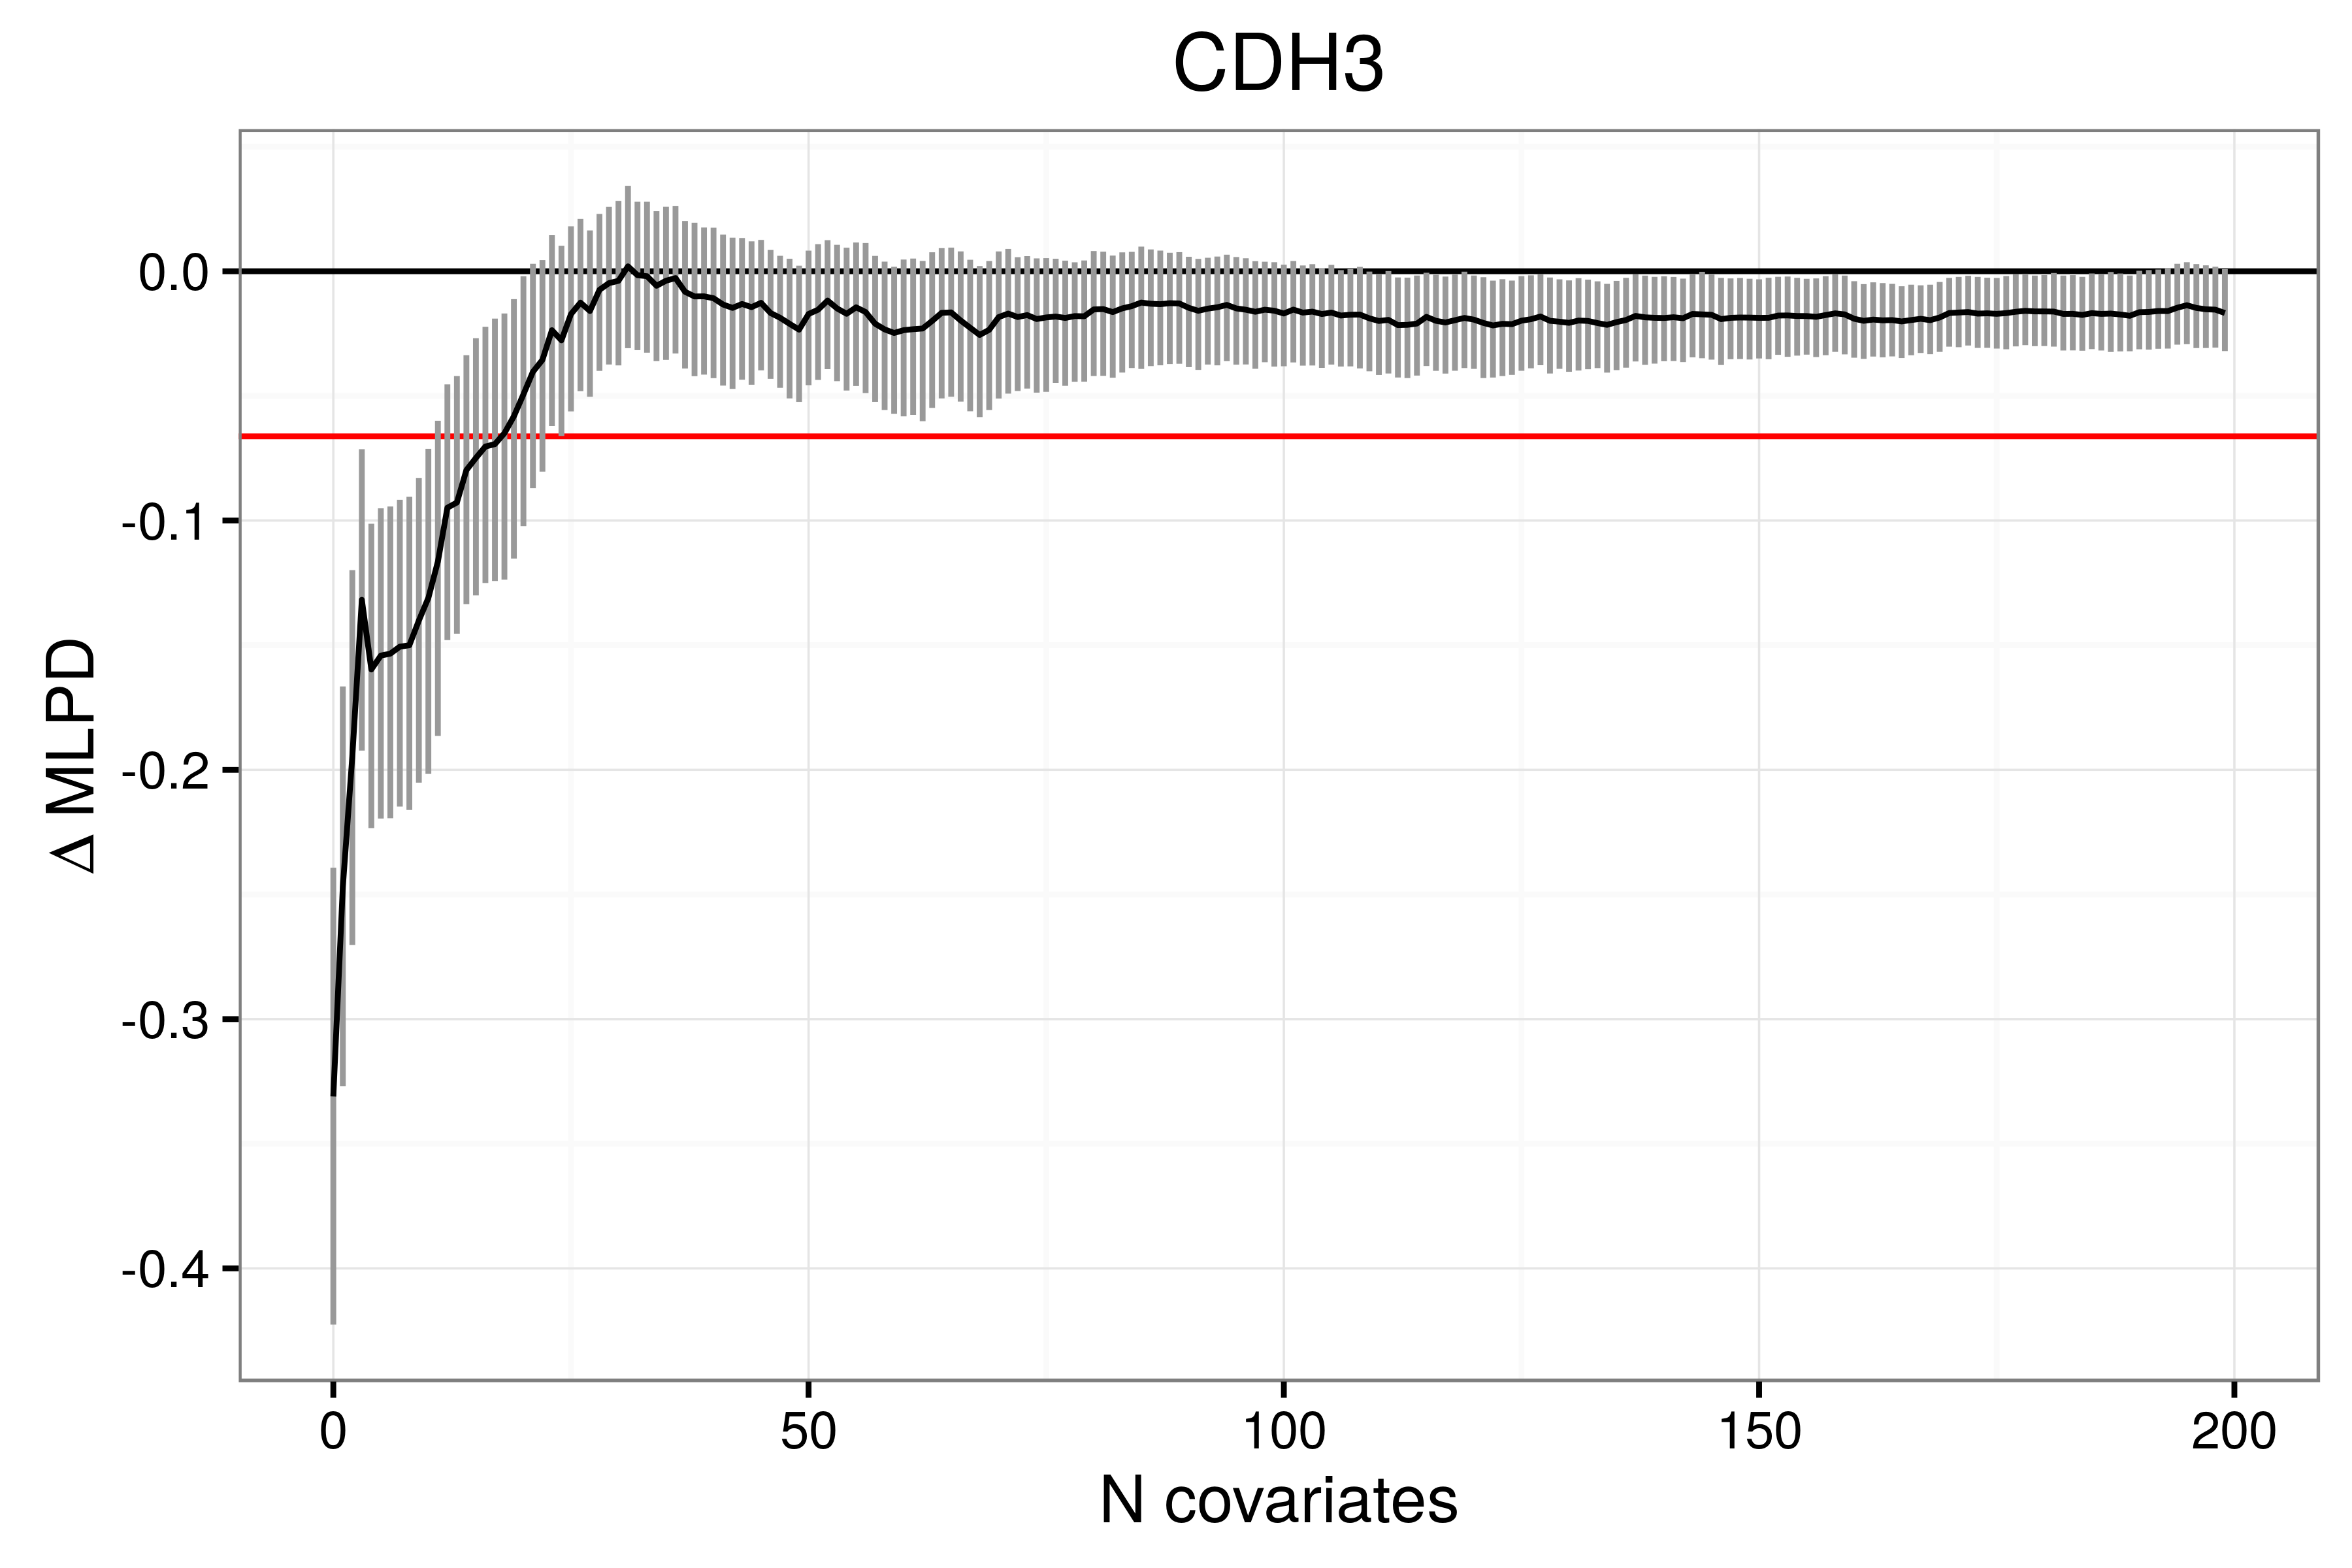
\includegraphics[width=1\linewidth]{figures/CDH3_CV_path.png}
  \end{subfigure}
  \begin{subfigure}{.48\textwidth}
    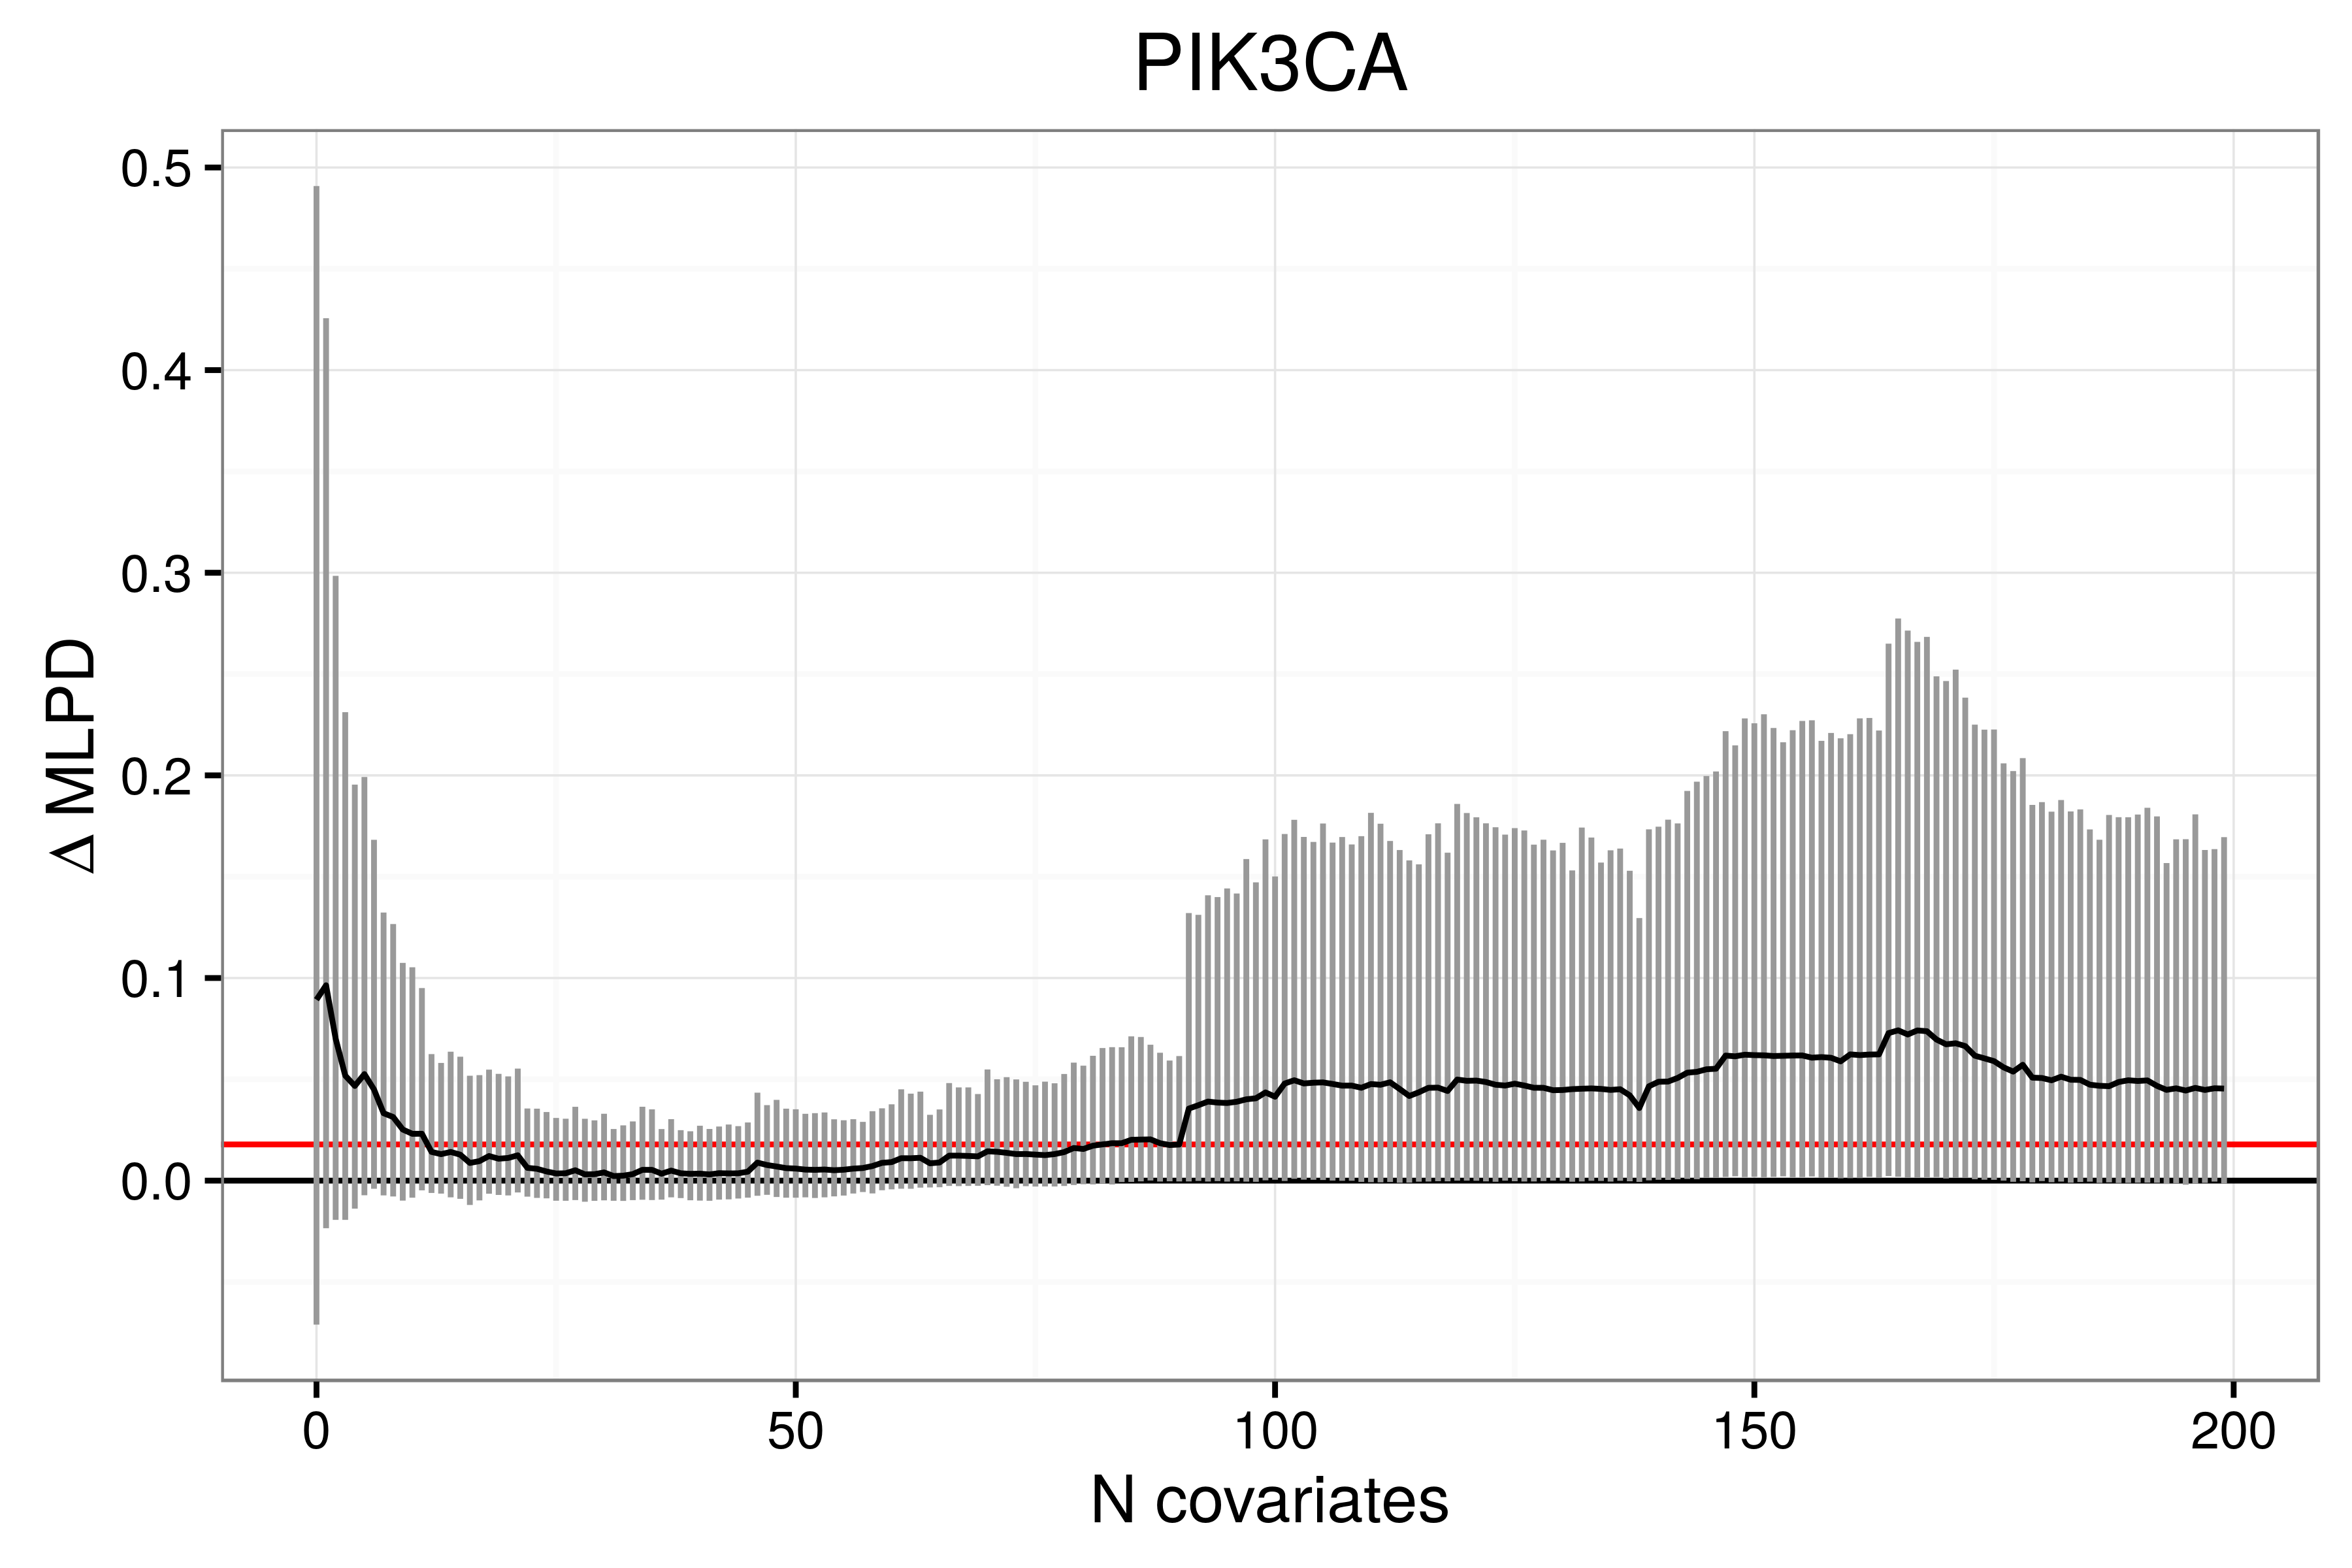
\includegraphics[width=1\linewidth]{figures/PIK3CA_CV_path.png}
  \end{subfigure}

  \caption{Predictive performance ($\Delta\textup{MLPD}$) of projected submodel $M_\perp$ during
  each step of the forward search in the model-size-selection phase. Two of the 105 models are shown.
  The black curve shows the median (corresponding to $\alpha = 0.50$) and
  gray lines the 95\% interval of $\Delta\textup{MLPD}$ computed with Bayesian bootstrap.
  The red line depicts the model-size selection threshold $U$ (with $\gamma=0.2$).
  The model size was chosen as the point where the black curve crosses the red line.
  The final \emph{CDH3} model (shown left) was one of the best performing ones,
  no model was found for \emph{PIK3CA} (shown right), as the intercept-only model
  already performed better than the full model.}
  \label{fig:forward-search}
\end{figure}

Projected models larger than approximately 28 miRNA variables performed
increasingly poorly as the model size increased. This is illustrated in Figure
\ref{fig:n-miRNAs-vs-R2}. A similar trend was observed by trying different
model-size threshold parameters $\alpha$ and $\gamma$ (data not shown).

\begin{figure}[!h]
  \centering
  \includegraphics[height=11cm]{figures/n_miRNAs_vs_R2.pdf}
  \caption{Size of final model compared to model goodness-of-fit. The x-axis corresponds to
  the total number of chosen miRNA variables in each final projected model (N miRNAs).
  The three y-axes show the number of significant miRNA variables (N significant miRNAs),
  $R^2$ of the projected model ($R_{\textup{full}}^2$), and the
  difference in $\bar{R}^2$ between the projected and gene-only models
  ($\Delta\bar{R}^2$). Higher values for the y-axes are better.
  Each point represents one model fitted for one gene. A
  small jitter has been added to the points on the x-axis to help visualize all of them.
  Curves were fitted with locally weighted scatter plot smoothing (LOESS) and
  shaded areas represent 95\% confidence interval. A trend can be seen, where
  models larger than approximately 28 included miRNAs perform increasingly poorly.}
  \label{fig:n-miRNAs-vs-R2}
\end{figure}

Lasso regression produced models with at least one miRNA for 74 genes, out of
which only 57 were common to the ones found by projection prediction (PPVS).
For 18 of the lasso models, the mRNA expression variable was excluded from
the chosen model.
Figure \ref{fig:model-size} shows a comparison of model size distribution
and $\Delta\bar{R}^2$ between PPVS and lasso.

\begin{figure}[!h]
  \centering
  \begin{subfigure}{.45\textwidth}
    \includegraphics[width=1\linewidth]{figures/R2comparison/n_miRNA_comparison.pdf}
  \end{subfigure}
  \begin{subfigure}{.45\textwidth}
    \includegraphics[width=1\linewidth]{figures/R2comparison/R2_comparison.pdf}
  \end{subfigure}

  \caption{Comparison of final model sizes (shown left) and 
      increase in proportion of protein variance explained
      compared to the gene-only model ($\Delta\bar{R}^2$, shown right) between
      projection prediction (PPVS) and lasso regression. PPVS models were slightly
      smaller on average (though the difference was not significant). The predictive
      performance of PPVS was better (as measured with $\Delta\bar{R}^2$).}
  \label{fig:model-size}
\end{figure}




\subsubsection*{Target prediction performance}

Considering each selected miRNA variable as a putative miRNA-mRNA target
interaction, PPVS generated a total 945 target predictions, out of which
253 were significant (on a 95\% posterior interval). Table \ref{table:final-models}
lists the significant predictions.
Lasso regression generated all together 650 target predictions. Figure
\ref{fig:venn} shows the overlap of predictions by PPVS and lasso, and also
that of significant predictions from PPVS and the same number of top
predictions from lasso, where lasso predictions were ranked by the absolute value of
the regression coefficient.\footnote{Lasso regression does not provide any
rank measures or tests of significance.}

\begin{figure}[!h]
  \centering
  \begin{subfigure}{.45\textwidth}
    \centering
    \includegraphics[width=1\linewidth]{figures/compareModels/Venn-PPVS-lasso.pdf}
  \end{subfigure}
  \begin{subfigure}{.45\textwidth}
    \centering
    \includegraphics[width=1\linewidth]{figures/compareModels/Venn-PPVS_sig-lasso_top.pdf}
  \end{subfigure}

  \caption{Venn diagrams showing the overlap of all target predictions from PPVS
  and lasso (shown left) and the overlap of significant (on the 95\% posterior) predictions
  from PPVS  and the same number of top predictions from lasso (ranked by
  absolute value of regression coefficient). There is very little overlap
  between the predictions made by the two methods. The proportion of overlap is
  slightly larger for the significant and top predictions.}
  \label{fig:venn}
\end{figure}

PPVS regression coefficients for miRNA covariates had larger magnitude (i.e. absolute value)
on average than lasso, for target interactions predicted by both, 
implying stronger miRNA effects on protein expression.
Correlation of the coefficients was
fairly high ($0.86$), and there were only three predicted targets for which
the methods did not agree on the sign of the coefficient. A scatter plot
comparing the coefficients of the common predictions is shown in Figure
\ref{fig:scatter-ppvs-lasso}.

\begin{figure}[htb]
  \centering
  \includegraphics[width=.8\linewidth]{figures/compareModels/Scatter-PPVS-lasso.pdf}
  \caption{Comparison of miRNA regression coefficients from projection
  prediction (PPVS, x-axis, posterior median) and lasso regression (y-axis) for the 145 targets predicted by both methods.
  Triangles are significant coefficients in PPVS. The gray line ($y=x$) corresponds to
  equal coefficients from the two methods. The coefficients from PPVS had
  larger magnitude on average, implying stronger miRNA effects on protein expression.
  cor: Pearson correlation between the coefficients.
  }
  \label{fig:scatter-ppvs-lasso}
\end{figure}

PPVS and lasso had similar performance in regards of discovering validated
targets; limiting predictions to the ones with most confidence did not
significantly increase the proportion of validated targets for either method.
Approximately 12\% of PPVS and 14\% of lasso predictions were present in the
union of TarBase and miRTarBase. These proportions were 13\% and 14\% for the
significant PPVS and top lasso predictions, respectively.

For both methods, approximately half of the coefficients for both all
predicted and validated targets were positive, indicating upregulation by the
miRNA. In contrast, in TarBase, all of the discovered validated interactions
were classified as suppressive. miRTarBase does not provide data on the
nature of the regulation.
